\documentclass[14pt,a4paper]{extarticle}
\usepackage{../templates/preamble}
\usepackage{amsmath}
\usepackage{amsfonts}

\newcommand{\reportof}{практической работе №5}
\newcommand{\theme}{Функции нескольких переменных}

\begin{document}
\begin{titlepage}
    \begin{center}
        {\bfseries
        МИНОБРНАУКИ РОССИИ\par
        САНКТ-ПЕТЕРБУРГСКИЙ ГОСУДАРСТВЕННЫЙ\par
        ЭЛЕКТРОТЕХНИЧЕСКИЙ УНИВЕРСИТЕТ\par
        <<ЛЭТИ>> ИМ. В.И. УЛЬЯНОВА (ЛЕНИНА)\par
        Кафедра \department

        \vspace{0.23\textheight}
        ОТЧЁТ\par
        по \reportof\par
        по дисциплине <<\discipline>>\par
        Тема: \theme
        \vspace{0.28\textheight}
        }
        \begin{table}[!ht]
            \begin{tabularx}{\textwidth}{p{60mm}X>{\centering\arraybackslash}p{45mm}}
                Студент гр. 4352 & \_\_\_\_\_\_\_\_\_\_\_\_\_\_\_\_\_\_\_\_ & {Даричев Е. М.} \\ [5.4mm]  % Line height
                Преподаватель    & \_\_\_\_\_\_\_\_\_\_\_\_\_\_\_\_\_\_\_\_ & {\teacher} \\ [5.4mm]
            \end{tabularx}
        \end{table}

        Санкт-Петербург\par
        \yyear
    \end{center}
\end{titlepage}
\setcounter{page}{2}

\section*{Цель работы}
        Изучить методы работы с функциями нескольких переменных.


\section*{Отчёт о проделанной работе}
В задании дана функция (\ref{eq:5.1.1}). После изучения методических материалов
с помощью функции plot3d в Jupyter Notebook был построен её график
(рис. \ref{pic:5.1.1}).

\begin{equation}\label{eq:5.1.1}
    f(x, y) = \sin{\sqrt{x^2 + y^2}}
\end{equation}
\begin{figure}[ht!]
    \centering
    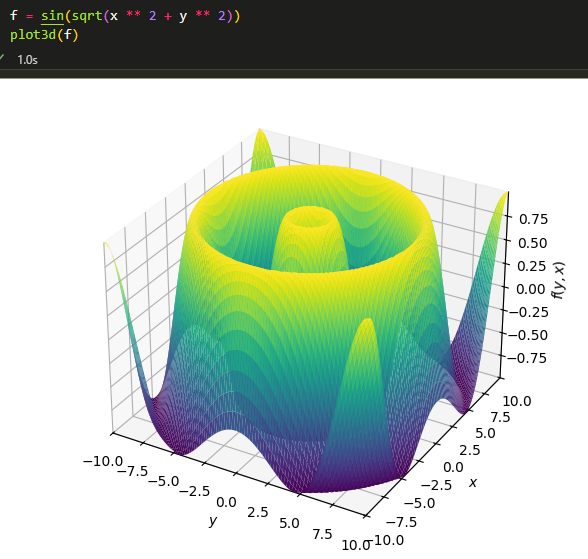
\includegraphics[width=0.6\linewidth]{figures/5.1/1.png}
    \caption{Задание 1.1}
    \label{pic:5.1.1}
\end{figure}
\newpage

        Далее дана функция (\ref{eq:5.1.2}). Теперь её надо
отобразить с ограничением на переменные. Сделаем это с помощью
дополнительных параметров (рис. \ref{pic:5.1.2}).

\begin{equation}
    \label{eq:5.1.2}
    f(x, y) = e ^ {-0.9x^2-0.45(x-y)^2}
\end{equation}
\begin{figure}
    [ht!]\centering
    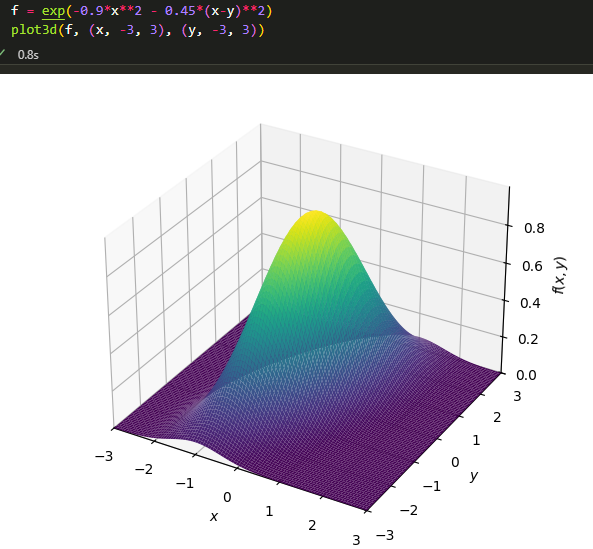
\includegraphics[width=\linewidth]{figures/5.1/2.png}
    \caption{Задание 1.2}
    \label{pic:5.1.2}
\end{figure}
\newpage


Построим следующий график функции (\ref{eq:5.1.3}) (рис \ref{pic:5.1.3}).

\begin{equation}
    \label{eq:5.1.3}
    f(x, y) = x \cos{y}
\end{equation}

\begin{figure}
    [ht!]\centering
    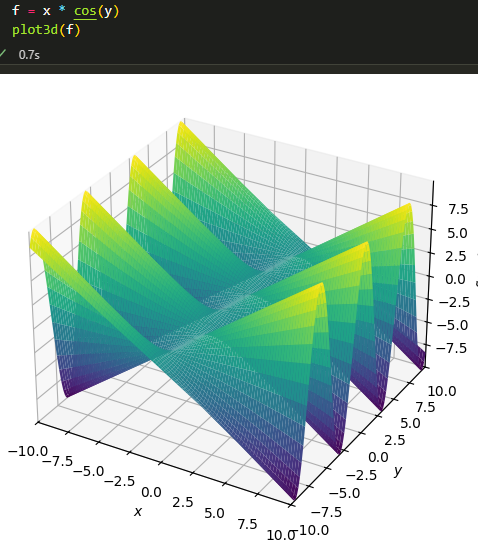
\includegraphics[width=\linewidth]{figures/5.1/3.png}
    \caption{Задание 1.3}
    \label{pic:5.1.3}
\end{figure}
\newpage


В следующем задании необходимо придумать математическую модель,
которая зависит от оценок (по пятибалльной шкале) трех членов
экспертной группы и возвращает вероятность принятия
положительного решения. В качестве функции взято обычное среднее
значение оценок, которое впоследствии нормализируется (рис. \ref{pic:5.1.4}).
Так как мы можем строить функции только от двух переменных,
то в качестве оценки эксперта 3 взята оценка 2.

\begin{figure}
    [ht!]\centering
    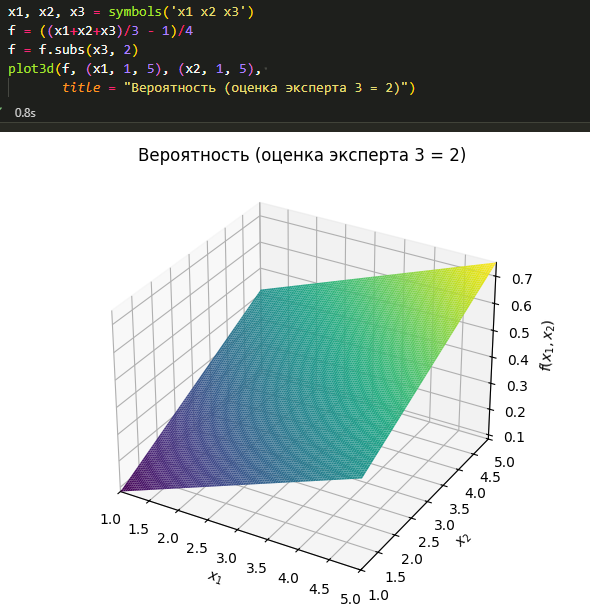
\includegraphics[width=\linewidth]{figures/5.1/4.png}
    \caption{Задание 1.4}
    \label{pic:5.1.4}
\end{figure}
\newpage

Следующая модель зависит от вероятности того, что пойдет дождь,
температуры за окном и оценки по десятибалльной шкале
заинтересованности данного человека некоторым мероприятием.
Возвращает значение 0, если человек не пойдет на это мероприятие,
и 1, если пойдет. Здесь мы перемножаем все факторы и сравниваем
его с некоторым пороговым значением вероятности (рис \ref{pic:5.1.5}).

\begin{figure}
    [ht!]\centering
    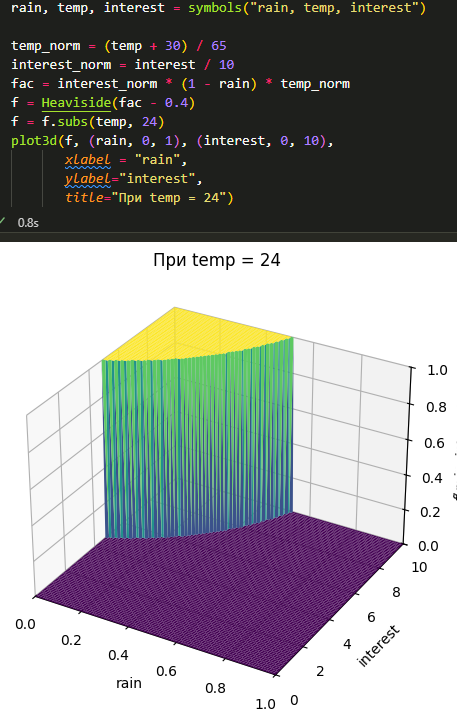
\includegraphics[width=0.8\linewidth]{figures/5.1/5.png}
    \caption{Задание 1.5}
    \label{pic:5.1.5}
\end{figure}
\newpage

Во втором задании необходимо построить графики функций (\ref{eq:5.2.1}-\ref{eq:5.2.3}), найти
их нули и построить графики нулей.

\begin{align}
    \label{eq:5.2.1}
    f(x, y) &= x(y - 5) ^ 2 \\
    \label{eq:5.2.2}
    f(x, y) &= (y - \frac{e}{20})^2 \sin(\pi x) \\
    \label{eq:5.2.3}
    f(x, y) &= x \sin (x) \sin(y - 2)
\end{align}

\begin{figure}
    [ht!]\centering
    \begin{subfigure}{0.48\linewidth}
        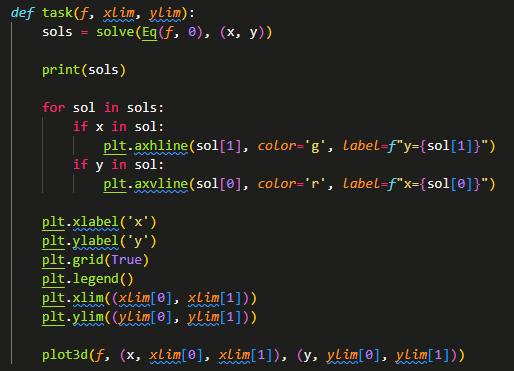
\includegraphics[width=0.95\linewidth]{figures/5.2/1.code.png}
        \caption{Код для выполнения}
        \label{pic:code}
    \end{subfigure}
    \begin{subfigure}{0.48\linewidth}
        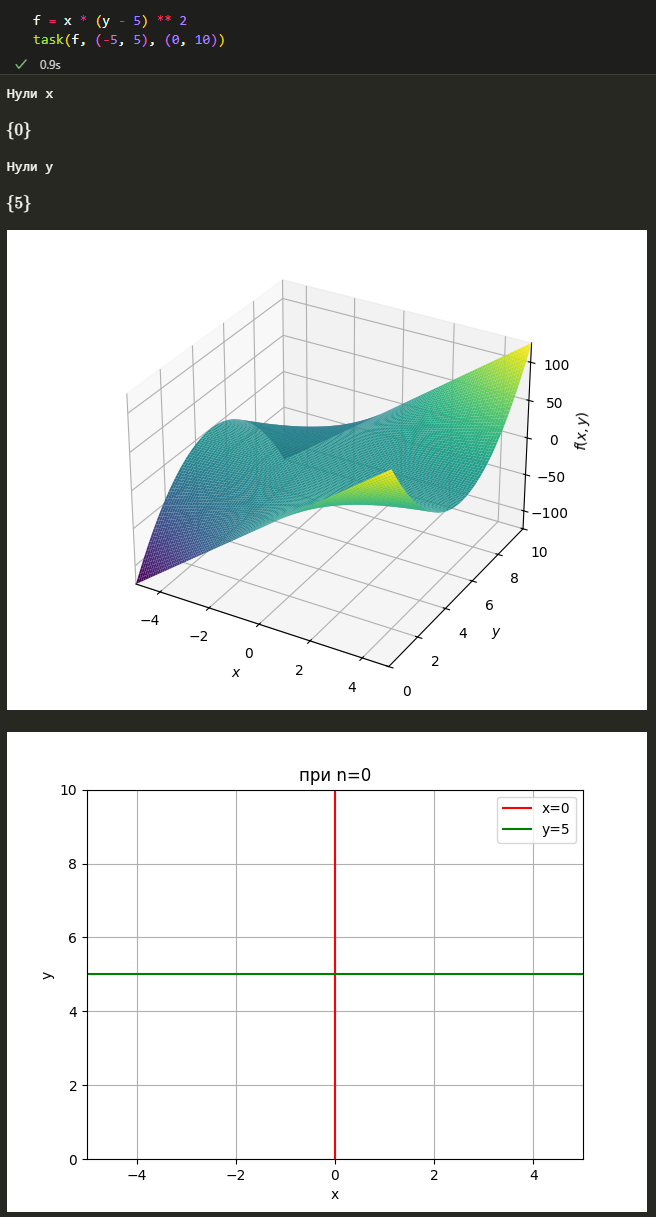
\includegraphics[width=0.95\linewidth]{figures/5.2/1.1.png}
        \caption{Формула \ref{eq:5.2.1}}
        \label{pic:5.2.1}
    \end{subfigure}
    \caption{Задание 2.1, певая часть}
\end{figure}\newpage
\begin{figure}
    [ht!]\centering
    \begin{subfigure}{0.48\linewidth}
        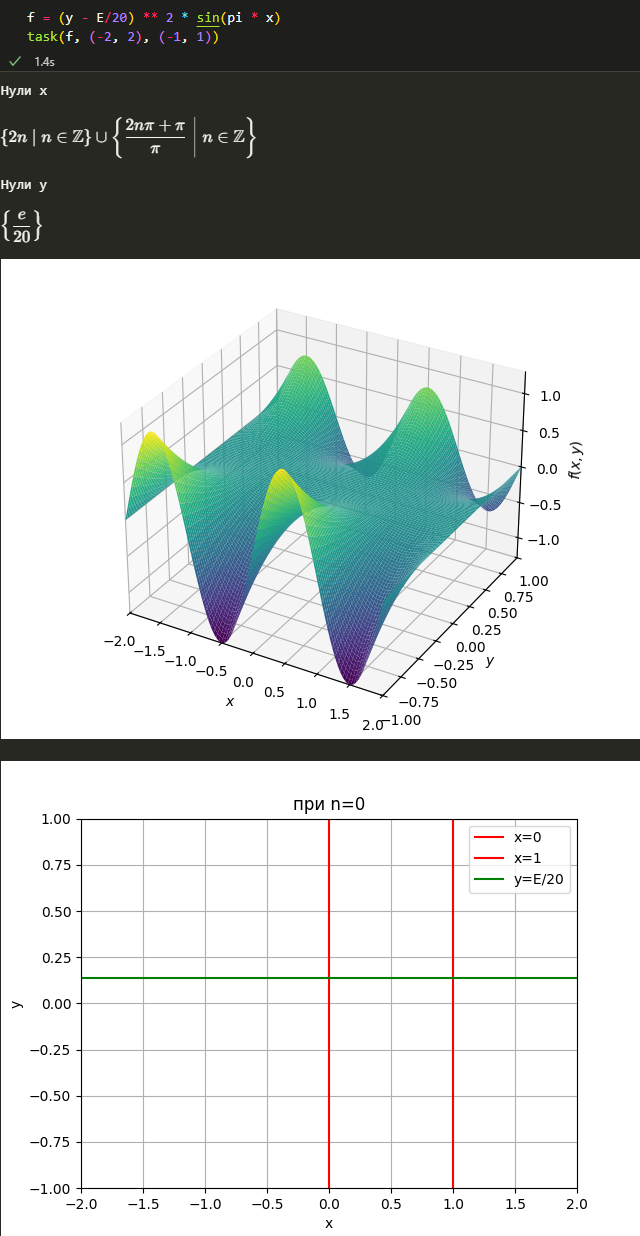
\includegraphics[width=0.95\linewidth]{figures/5.2/1.2.png}
        \caption{Формула \ref{eq:5.2.2}}
        \label{pic:5.2.2}
    \end{subfigure}
    \begin{subfigure}{0.48\linewidth}
        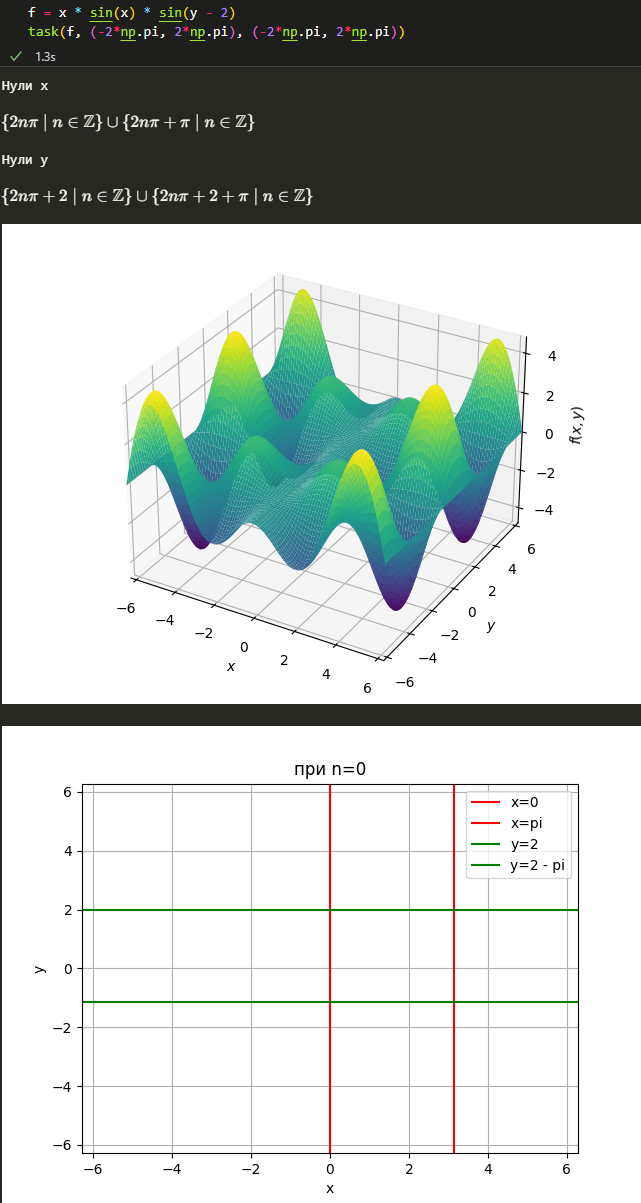
\includegraphics[width=0.95\linewidth]{figures/5.2/1.3.png}
        \caption{Формула \ref{eq:5.2.3}}
        \label{pic:5.2.3}
    \end{subfigure}
    \caption{Задание 2.1, вторая часть}
\end{figure}

Для функции (\ref{eq:5.2.1}):
\begin{itemize}
    \item Нули $x$:
    $\displaystyle \left\{0\right\}$
    \item Нули $y$:
    $\displaystyle \left\{5\right\}$
\end{itemize}

Для функции (\ref{eq:5.2.2}):
\begin{itemize}
    \item Нули $x$:
    $\displaystyle \left\{2 n\; \middle|\; n \in \mathbb{Z}\right\} \cup \left\{\frac{2 n \pi + \pi}{\pi}\; \middle|\; n \in \mathbb{Z}\right\} = \left\{n \;\middle|\; n \in \mathbb{Z}\right\}$ 
    \item Нули $y$:
    $\displaystyle \left\{\frac{e}{20}\right\}$
\end{itemize}

Для функции (\ref{eq:5.2.3}):
\begin{itemize}
    \item Нули $x$:
    $\displaystyle \left\{2 n \pi\; \middle|\; n \in \mathbb{Z}\right\} \cup \left\{2 n \pi + \pi\; \middle|\; n \in \mathbb{Z}\right\} = \left\{n\pi \;\middle|\; n \in \mathbb{Z}\right\}$
    \item Нули $y$:
    $\displaystyle \left\{2 n \pi + 2\; \middle|\; n \in \mathbb{Z}\right\} \cup \left\{2 n \pi + 2 + \pi\; \middle|\; n \in \mathbb{Z}\right\} = \left\{n\pi + 2 \;\middle|\; n \in \mathbb{Z}\right\}$
\end{itemize}

Задание 1. Описание функции и поиск размерности
гиперплоскости.
1. Дана функция \(f(x_1, x_2, x_3, x_4) = a_4 x_4 + a_3 x_3 + a_2 x_2 + a_1 x_1 + a_0\)
Данная функция отвечает на вопрос: «Является ли текст спамом?»
Если является, функция возвращает 1, если нет — 0. Переменная
$x_1$ равна количеству упоминаний в тексте одной из форм слова 
«покупать». Переменная $x_2$ равна 1, если в тексте есть слово
«скидка», и 0 — в противном случае. Переменная $x_3$ равна 1,
если в тексте есть слово «акция» и 0 — в противном случае.
$x_4$ равна длине текста в словах.

Описание: $f : \mathbb{R} \times\{0, 1\}\times\{0, 1\}\times\mathbb{R} \rightarrow \{0, 1\}$
Для задания гиперплоскости необходим порог.
\begin{equation*}
    f(x_1, x_2, x_3, x_4) > r
\end{equation*}

Это неравенство определяет плоскость в четырехмерном пространстве
признаков. Размерность плоскости на единицу меньше размерности
пространства, в котором она находится. Значит, размерность равна 3.

2. Дана функция \(f(x_1, x_2, x_3) = a_3 x_3 + a_2 x_2 + a_1 x_1 + a_0\)
Данная функция отвечает на вопрос: «С какой вероятностью клиент
сделает вклад?» Переменная $x_1$ равна количеству раз, которое клиент
делал вклады ранее. Переменная $x_2$ равна сумме всех этих вкладов.
Переменная $x_3$ равна 1, если у клиента есть вклад в данный момент,
и 0 — в противном случае.

Описание: $f: \mathbb{R}^2 \times \{0, 1\} \rightarrow [0, 1] $

Для задания гиперплоскости необходим порог.
\begin{equation*}
    f(x_1, x_2, x_3) > r
\end{equation*}

Это неравенство определяет плоскость в трехмерном пространстве
признаков. Размерность плоскости на единицу меньше размерности
пространства, в котором она находится. Значит, размерность равна 2.

3. Дана функция \(f(x_1, x_2, x_3, x_4) = a_4 x_4 + a_3 x_3 + a_2 x_2 + a_1 x_1 + a_0\)
Данная функция отвечает на вопрос: «Болен ли пациент гриппом?»
Переменная $x_1$ равна 1, если пациент привит от гриппа, и 0 — в
противном случае. Переменная $x_2$ равна температуре пациента.
Переменная $x_3$ равна 1, если у пациента есть кашель, и 0 — в
противном случае. $x_4$ равна 1, если у пациента есть насморк,
и 0 — в противном случае.

Описание: $f: \{0, 1\}\times [34, 44]\times\{0, 1\}\times\{0, 1\} \rightarrow \{0, 1\} $

Для задания гиперплоскости необходим порог.
\begin{equation*}
    f(x_1, x_2, x_3, x_4) > r
\end{equation*}

Это неравенство определяет плоскость в четырёхмерном пространстве
признаков. Размерность плоскости на единицу меньше размерности
пространства, в котором она находится. Значит, размерность равна 3.

\section*{Вывод}
В ходе выполнения работы мы изучили методы работы с функциями нескольких
переменных, научились находить нули таких функций и отображать их в виде
графиков нулей.
\end{document}